\documentclass{article}

\usepackage{graphicx}
\usepackage{tikz}
\usepackage{tikzsymbols}
\usetikzlibrary{calc,patterns,shapes.geometric}
\pagestyle{empty}
\usepackage[margin=0pt]{geometry}
\geometry{papersize={14in,12in}}

\def\centerarc[#1](#2)(#3:#4:#5){\draw[#1] ($(#2)+({#5*cos(#3)},{#5*sin(#3)})$) arc (#3:#4:#5);}

\begin{document}
	\begin{figure}
		\centering
		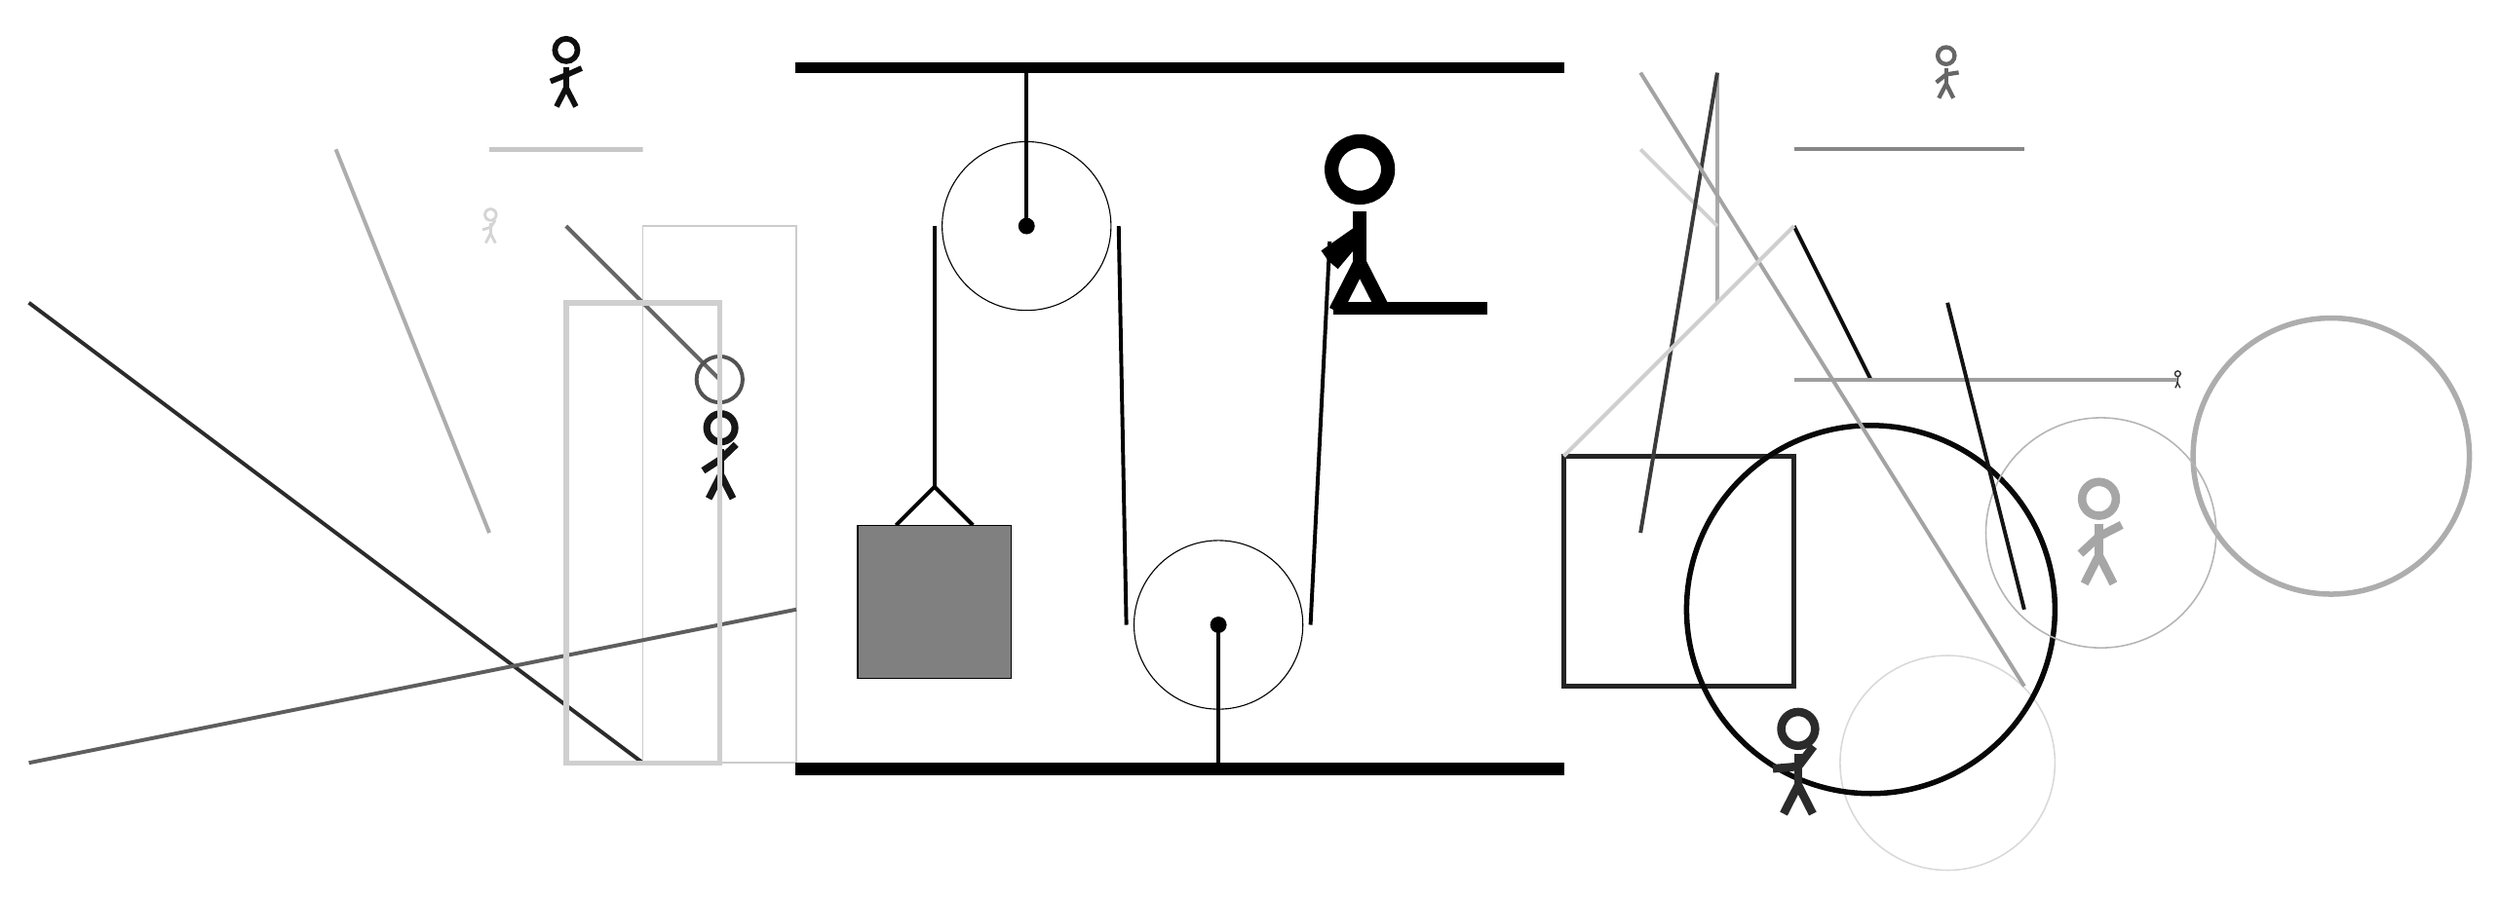
\begin{tikzpicture}
			%%%%% START %%%%%
			
			\draw[fill=black] (-2, 9) rectangle (8, 9.125);
			
			\draw (3.5, 1.8) circle (1.1);
			\draw[fill=black] (3.5, 1.8) circle (0.1);
			\draw[line width=0.5mm] (3.5, 1.8) -- (3.5, 0);
			
			\draw (1, 7) circle (1.1);
			\draw[fill=black] (1, 7) circle (0.1);
			\draw[line width=0.5mm] (1, 9) -- (1, 7);
			
			\draw[line width=0.5mm](-0.7, 3.1) --  (-0.2, 3.6) -- (0.3, 3.1);
			\draw[fill=black!50] (-1.2, 3.1) rectangle (0.8, 1.1);
			
			\draw [line width=0.2mm, color=black!15](13, 0) circle (1.4);
			
			\draw[line width=0.5mm, color=black!83](-4, 0) -- (-12, 6);
			\draw [line width=0.7mm, color=black!32](18, 4) circle (1.8);
			\node[line width=0.6mm, color=black!17] at (-6, 7) {\Strichmaxerl[2][17][57]};
			\draw[line width=0.5mm, color=black!95](12, 5) -- (11, 7);
			
			\draw[line width=0.6mm, color=black!22] (-4, 8) rectangle (-6, 8);
			\draw[line width=0.2mm, color=black!20] (-2, 0) rectangle (-4, 7);
			
			\draw[line width=0.5mm, color=black!54] (10, 6) rectangle (10, 6);
			\draw[line width=0.5mm, color=black!33](10, 6) -- (10, 9);
			\node[line width=0.5mm, color=black!91] at (-3, 4) {\Strichmaxerl[5][33][44]};
			\draw[line width=0.6mm, color=black!86] (8, 1) rectangle (11, 4);
			\draw[line width=0.5mm, color=black!18](10, 7) -- (9, 8);
			\draw[line width=0.5mm, color=black!77](9, 3) -- (10, 9);
			
			\draw[line width=0.5mm, color=black!60](-3, 5) -- (-5, 7);
			\node[line width=0.6mm, color=black!78] at (16, 5) {\Strichmaxerl[1][78][85]};
			\draw [line width=0.7mm, color=black!97](12, 2) circle (2.4);
			
			\node[line width=0.6mm, color=black!35] at (15, 3) {\Strichmaxerl[6][43][27]};
			
			\draw[line width=0.5mm, color=black!36](9, 9) -- (14, 1);
			\draw [line width=0.5mm, color=black!68](-3, 5) circle (0.3);
			
			\draw[line width=0.5mm, color=black!32](-6, 3) -- (-8, 8);
			\draw[line width=0.5mm, color=black!47](11, 8) -- (14, 8);
			\draw [line width=0.2mm, color=black!29](15, 3) circle (1.5);
			\draw[line width=0.5mm, color=black!38](11, 5) -- (16, 5);
			\node[line width=0.3mm, color=black!83] at (11, 0) {\Strichmaxerl[6][5][53]};
			\node[line width=0.4mm, color=black!94] at (-5, 9) {\Strichmaxerl[4][22][24]};
			\node[line width=0.4mm, color=black!60] at (13, 9) {\Strichmaxerl[3][39][9]};
			\draw[line width=0.5mm, color=black!92](13, 6) -- (14, 2);
			\draw[line width=0.5mm, color=black!63](-2, 2) -- (-12, 0);
			\draw[line width=0.7mm, color=black!19] (-3, 6) rectangle (-5, 0);
			
			\draw[line width=0.5mm, color=black!19](11, 7) -- (8, 4);
			
			\draw[line width=0.5mm](-0.2, 7) -- (-0.2, 3.6);
			\centerarc[line width=0.5mm](1, 7)(180:0:1.2000000000000002)
			\draw[line width=0.5mm](2.2, 7) -- (2.3, 1.8);
			\centerarc[line width=0.5mm](3.5, 1.8)(180:360:1.2000000000000002)
			\draw[line width=0.5mm](4.7, 1.8) -- (4.95, 6.8);
			
			\node at (5.3, 7) {\Strichmaxerl[10][35][-130]};
			\draw[fill=black] (5, 6) rectangle (7, 5.85);
			
			\draw[fill=black] (-2, 0) rectangle (8, -0.15);
			
			%%%%% END %%%%%
		\end{tikzpicture}
	\end{figure}	
\end{document}